
\section{Axes \& Legends}

\textit{All of the below can be set in styles rather than set on each plot or axis. $\exists$ a number of pre-fab styles for axes, lines, ticks, legends, and colorbars, such as: }\href{\docurl\#pgfp./pgfplots/every:major:tick}{\opt{every major tick}}, \href{\docurl\#pgfp./pgfplots/title:style}{\opt{title style}}, \href{\docurl\#pgfp./pgfplots/every:loglog:axis}{\opt{every loglog axis}}\textit{, etc. See \href{\docurl\#pgfp./pgfplots/every:axis}{\ul{here}} for a full list. Or, ideally, create your own style, appending it to the relevant elements as call for using: }\texttt{\textbackslash pgfplotsset\{ <style\_name>/.style=\dots\}}\textit{.}



%%%%%%%%%%%%%%%%%%%%%%%%%%%%%%%%%%%%%%%%%%%%%%%%%
\subsection*{Axis Lines \& Labels}

\textit{The following options afford setting axis and plot titles, including their style and positioning.}

\begin{multicols}{2}
{\footnotesize \color{blue}
\begin{itemize}[leftmargin=1mm,label={}]
    \item \href{\docurl\#pgfp./pgfplots/title}{title}
    \item \href{\docurl\#pgfp./pgfplots/extra:description}{extra description}
    \item \href{\docurl\#pgfp./pgfplots/axis:lines}{axis lines}
    \item \href{\docurl\#pgfp./pgfplots/axis:lines}{axis lines*}
    \item \href{\docurl\#pgfp./pgfplots/axis:x:line}{axis [x|y|z] line}
    \item \href{\docurl\#pgfp./pgfplots/axis:x:line*}{axis [x|y|z] line*}
    \item \href{\docurl\#pgfp./pgfplots/every:inner:x:axis:line}{every inner [x|y|z] line}
    \item \href{\docurl\#pgfp./pgfplots/every:outer:x:axis:line}{every outer [x|y|z] line}
    \item \href{\docurl\#pgfp./pgfplots/axis:line:style}{axis line style}
    \item \href{\docurl\#pgfp./pgfplots/x:axis:line:style}{{[x|y|z]} axis line style}
    \item \href{\docurl\#pgfp./pgfplots/every:boxed:x:axis}{every boxed [x|y|z] axis}
    \item \href{\docurl\#pgfp./pgfplots/separate:axis:lines}{separate axis lines}
    \item \href{\docurl\#pgfp./pgfplots/axis:x:line:shift}{axis [x|y|z] line shift}
    \item \href{\docurl\#pgfp./pgfplots/axis:x:discontinuity}{axis [x|y|z] discont\textquotesingle y}
    \item \href{\docurl\#pgfp./pgfplots/hide:x:axis}{hide [x|y|z] axis}
    \item \href{\docurl\#pgfp./pgfplots/inner:axis:line:style}{inner axis line style}
    \item \href{\docurl\#pgfp./pgfplots/outer:axis:line:style}{outer axis line style}
    \item \href{\docurl\#pgfp./pgfplots/grid}{grid}
    \item \href{\docurl\#pgfp./pgfplots/domain}{domain}
    \item {[x|y|z]}[min|max]
    \item \href{\docurl\#pgfp./pgfplots/xlabel}{{[x|y|z]}label}
    \item \href{\docurl\#pgfp./pgfplots/label:shift}{{[x|y|z]}label shift}
    \item {[x|y|z]}label near ticks
    \item \href{\docurl\#pgfp./pgfplots/xlabel:absolute}{{[x|y|z]}label absolute}
    \item \href{\docurl\#pgfp./pgfplots/axis:line:style}{\footnotesize axis line style}
    \item \href{\docurl\#pgfp./pgfplots/legend:pos}{legend pos}
    \item \href{\docurl\#pgfp./pgfplots/enlargelimits}{enlargelimits}
\end{itemize}
}
\end{multicols}

\begin{comment}
\textit{The following styles\textsuperscript{S} are available:}\\
{\color{blue}
\begin{minipage}[t]{3.0cm}
    \href{\docurl\#pgfp./pgfplots/every:axis}{every axis}\\
    \href{\docurl\#pgfp./pgfplots/every:semilogx:axis}{every semilogx axis}\\
    \href{\docurl\#pgfp./pgfplots/every:linear:axis}{every linear axis}\\
    \href{\docurl\#pgfp./pgfplots/every:axis:plot:post}{every axis plot post}\\
    \href{\docurl\#pgfp./pgfplots/every:forget:plot}{every forget plot}\\
    \href{\docurl\#pgfp./pgfplots/label:style}{label style}\\
    \href{\docurl\#pgfp./pgfplots/x:label:style}{{[x|y|z]} label style}\\
    \href{\docurl\#pgfp./pgfplots/title:style}{title style}\\
\end{minipage}
\begin{minipage}[t]{3.0cm}
    \href{\docurl\#pgfp./pgfplots/every:axis:post}{every axis post}\\
    \href{\docurl\#pgfp./pgfplots/every:loglog:axis}{every loglog axis}\\
    \href{\docurl\#pgfp./pgfplots/every:axis:plot}{every axis plot}\\
    \href{\docurl\#pgfp./pgfplots/every:axis:plot:no\#}{every axis plot no \#}\\
    \href{\docurl\#pgfp./pgfplots/every:axis:label}{every axis label}\\
    \href{\docurl\#pgfp./pgfplots/every:axis:x:label}{every axis x label}\\
    \href{\docurl\#pgfp./pgfplots/every:axis:title}{every axis title}\\
\end{minipage}}
\end{comment}


%%%%%%%%%%%%%%%%%%%%%%%%%%%%%%%%%%%%%%%%%%%%%%%%%
\subsection*{\href{\docurl\#pgfp./pgfplots/xtick:distance}{Tick Marks}}

\begin{multicols}{2}
{\footnotesize \color{blue}
\begin{itemize}[leftmargin=1mm,label={}]
    \item \href{\docurl\#pgfp./pgfplots/xtick}{{[x|y|z]}tick}
    \item \href{\docurl\#pgfp./pgfplots/xticklabel}{{[x|y|z]}ticklabel}
    \item \href{\docurl\#pgfp./pgfplots/xticklabels}{{[x|y|z]}ticklabels}
    \item \href{\docurl\#pgfp./pgfplots/xticklabels:from:table}{\textquotesingle\textquotesingle\textquotesingle\  from table}
    \item \href{\docurl\#pgfp./pgfplots/extra:xtick:label}{extra [x|y|z]tick label}
    \item \href{\docurl\#pgfp./pgfplots/xminorticks}{{[x|y|z]}minorticks}
    \item \href{\docurl\#pgfp./pgfplots/xmajorticks}{{[x|y|z]}majorticks}
    \item \href{\docurl\#pgfp./pgfplots/xtickmin}{{[x|y|z]}tickmin}
    \item \href{\docurl\#pgfp./pgfplots/xtickmax}{{[x|y|z]}tickmax}
    \item \href{\docurl\#pgfp./pgfplots/xtick:pos}{{[x|y|z]}tick pos}
    \item \href{\docurl\#pgfp./pgfplots/xticklabel:pos}{{[x|y|z]}ticklabel pos}
    \item \href{\docurl\#pgfp./pgfplots/xtick:align}{{[x|y|z]}tick align}
    \item \href{\docurl\#pgfp./pgfplots/xtick:distance}{{[x|y|z]}tick distance}
    \item \href{\docurl\#pgfp./pgfplots/xticklabel:shift}{{[x|y|z]}ticklabel shift}
    \item \href{\docurl\#pgfp./pgfplots/xticklabel:style}{{[x|y|z]}ticklabel style}
    \item \href{\docurl\#pgfp./pgfplots/minor:x:tick}{minor [x|y|z] tick\textsuperscript{S}}
    \item \href{\docurl\#pgfp./pgfplots/minor:x:tick:num}{minor [x|y|z] tick num}
    \item \href{\docurl\#pgfp./pgfplots/extra:x:ticks}{extra [x|y|z] ticks}
    \item \href{\docurl\#pgfp./pgfplots/xtickten}{{[x|y|z]}tickten}
    \item \href{\docurl\#pgfp./pgfplots/scaled:x:ticks}{scaled {[x|y|z]} ticks}
    \item \href{\docurl\#pgfp./pgfplots/max:space:between:ticks}{max space between ticks}
    \item \href{\docurl\#pgfp./pgfplots/min:space:between:ticks}{min space between ticks}
    \item \href{\docurl\#pgfp./pgfplots/try:min:ticks}{try min ticks}
    \item \href{\docurl\#pgfp./pgfplots/tickwidth}{tickwidth}
    \item \href{\docurl\#pgfp./pgfplots/major:tick:length}{major tick length}
    \item \href{\docurl\#pgfp./pgfplots/minor:tick:length}{minor tick length}
    \item \href{\docurl\#pgfp./pgfplots/subtickwidth}{subtickwidth}
    \item \href{\docurl\#pgfp./pgfplots/xtick:placement:tolerance}{{[x|y|z]}tick placement tolerance}
    \item \href{\docurl\#pgfp./pgfplots/hide:obscured:x:ticks}{{\footnotesize hide obscured {[x|y|z]} ticks}}
    \item \href{\docurl\#pgfp./tikz/sloped:like:y:axis}{sloped like [x|y|z] axis}
    \item \href{\docurl\#pgfp./pgfplots/every:x:tick:scale:label}{every x tick scale label}
\end{itemize}
}
\end{multicols}




%%%%%%%%%%%%%%%%%%%%%%%%%%%%%%%%%%%%%%%%%%%%%%%%%%%
\subsection*{\href{\docurl\#pgfp./pgfplots/view}{3D Axes}}




%%%%%%%%%%%%%%%%%%%%%%%%%%%%%%%%%%%%%%%%%%%%%%%%%%%%
\subsection*{\href{\docurl\#pgfp.polar}{Radial Axes}}




%%%%%%%%%%%%%%%%%%%%%%%%%%%%%%%%%%%%%%%%%%%%%%%%%%%%
\subsection*{\href{\docurl\#pgfp.back/addlegendentry}{Legends}}

\textit{Create imperatively using }\href{\docurl\#pgfp.back.addlegendentry}{\opt{\textbackslash addlegendentry}}\textit{ or }\href{\docurl\#pgfp/back/legend}{\opt{\textbackslash legend}}\textit{, or declaratively with option }\href{\docurl\#pgfp./pgfplots/legend:entries}{\opt{legend entries}}\textit{. Behind scenes, legends are implemented as Tikz matrices, so the styling for those apply here as well. Customize placement \& appearance:}

{\color{blue}
\begin{minipage}[t]{3.0cm}
\href{\docurl\#pgfp./pgfplots/at}{at}\\
\href{\docurl\#pgfp./pgfplots/anchor}{anchor}\\
\href{\docurl\#pgfp./pgfplots/legend:pos}{legend pos}\\
\href{\docurl\#pgfp./pgfplots/mesh:legend}{mesh legend}\\
\href{\docurl\#pgfp./pgfplots/reverse:legend}{reverse legend}
\end{minipage}
\begin{minipage}[t]{3.0cm}
\href{\docurl\#pgfp./pgfplots/}{{[x|y|z]}bar legend}\\
\href{\docurl\#pgfp./pgfplots/}{{[x|y|z]}bar inverval legend}\\
\href{\docurl\#pgfp./pgfplots/}{legend plot pos}\\
\href{\docurl\#pgfp./pgfplots/}{legend cell align}\\
\href{\docurl\#pgfp./pgfplots/}{legend columns}\\
\href{\docurl\#pgfp./pgfplots/}{transpose legend}
\end{minipage}}

\begin{comment}
\textit{The following styles\textsuperscript{S} are available:}
{\color{blue}
\begin{minipage}[t]{3.6cm}
\href{\docurl\#pgfp./pgfplots/legend:style}{legend style}\\
\href{\docurl\#pgfp./pgfplots/every:legend:image:post}{every legend image post}\\
\href{\docurl\#pgfp./pgfplots/legend:image:post:style}{legend image post style}
    every axis legend\\
    every axis image post\\
    every legend to name picture\\
\end{minipage}
\begin{minipage}[t]{2.6cm}
\href{\docurl\#pgfp./pgfplots/line:legend}{line legend}\\
\href{\docurl\#pgfp./pgfplots/empty:legend}{empty legend}\\
\href{\docurl\#pgfp./pgfplots/area:legend}{area legend}\\
\href{\docurl\#pgfp./pgfplots/every:axis:legend}{every axis legend}
    legend style\\
    legend image post style\\
\end{minipage}}
\end{comment}


%%%%%%%%%%%%%%%%%%%%%%%%%%%%%%%%%%%%%%%%%%%%%%%%%%%
\subsection*{\href{\docurl\#pgfp./pgfplots/colorbar}{Colorbars}}

\begin{wrapfigure}[5]{r}{2.2cm}
\vspace{-8mm}
\resizebox{2cm}{!}{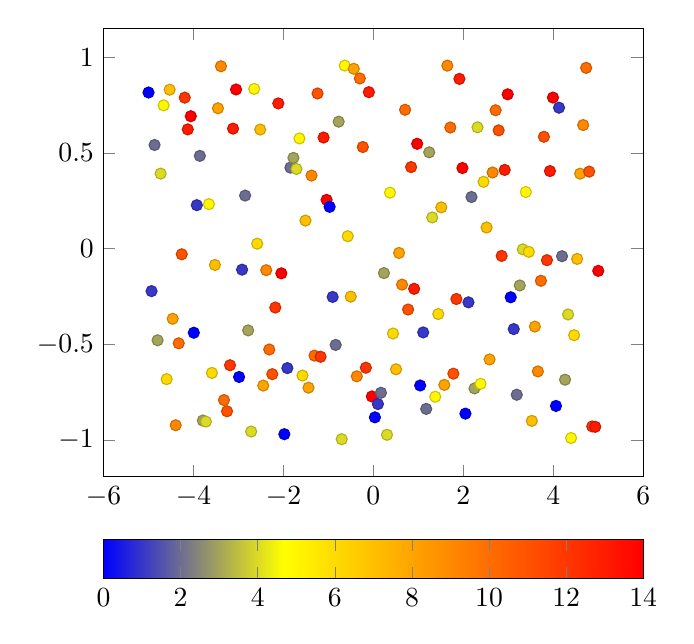
\begin{tikzpicture}
\begin{axis}[colorbar horizontal]
    \addplot[only marks,scatter,scatter src={mod(\coordindex,15)},samples=150,] {rand};
\end{axis}
\end{tikzpicture}}
\end{wrapfigure}

\textit{These can be positioned, given different color scales, [dis]connected to plotting variables, moved outside an individual plot, etc. Often associated with }\href{\docurl\#pgfp./pgfplots/point:meta}{\opt{point meta}}\textit{ data.}

{\color{blue}
\begin{minipage}[t]{3.0cm}
colorbar right\\
colorbar top\\
colorbar horizontal\\
every colorbar\\ 
point meta [min|max]\\
colorbar to name
\end{minipage}
\begin{minipage}[t]{3.0cm}
colorbar shift\\
colorbar style\\
colorbar/width\\
colorbar source\\
colorbar sampled\\
colorbar as legend
\end{minipage}}



%%%%%%%%%%%%%%%%%%%%%%%%%%%%%%%%%%%%%%%%%%%%%%%%%
\subsection*{\href{\docurl\#pgfp.axis:description:cs}{Axis Coordinate Systems}}

\textit{$\exists$ two coordinate systems, unique to PGFPlots that allow node positioning along axis locations, namely, }\href{\docurl\#pgfp./pgfplots/axis:description:cs}{\opt{axis description cs}}\textit{ and }\href{\docurl\#pgfp./xticklabel:cs}{\opt{[x|y|z]ticklabel cs}}\textit{. The former is simple, the latter affords better placement along 3D axes. Additionally, these coordinate systems enable some extra anchors for nodes: }\texttt{\href{\docurl\#pgfp.near:xticklabel}{near [x|y|z]ticklabel}}, \texttt{\href{\docurl\#pgfp.near:xticklabel:opposite}{near ticklabel opposite}}.
